% !TEX encoding = UTF-8 Unicode
% -*- coding: UTF-8; -*-
% vim: set fenc=utf-8

\section{Autentizace}\label{sec:autentizace}

Autentizace (anglicky authentication) je proces určení skutečné identity uživatele.
Pro webové aplikace se nejčastěji jedná o klasické přihlášení uživatele do aplikace pod svým uživatelským účtem.
K autentizaci lze nejčastěji rozdělit na dva způsoby, stavovou a bezstavovou autentizace.

\subsection{Stavová autentizace}\label{subsec:stavováAutentizace}
Stavová autentizace (viz diagram na obrázku~\ref{fig:statefullAuthentication}) je nejčastější způsob autentizace na internetu.
Tento způsob je velmi jednoduchý na implementaci a díky své oblíbenosti lze jeho implementaci najít v každé větší webové knihovně, či frameworku.

Server si musí pamatovat uložená data pro všechny přihlášené uživatele (nejčastěji v Session), ale také klient si musí pamatovat identifikátor těchto dat pomocí (nejčastěji v Cookies).
Pro správné fungování stavová autentizace potřebuje, aby se všechny části aplikace, které potřebují přístup k informacím o přihlášeném uživateli, nacházeli na stejné doméně.
Toto omezení vyplývá z použití cookies na straně klienta a bezpečnostním opatřením ze strany prohlížeče ohledně přístupu k nim.

\begin{figure}[ht!]
    \centering
    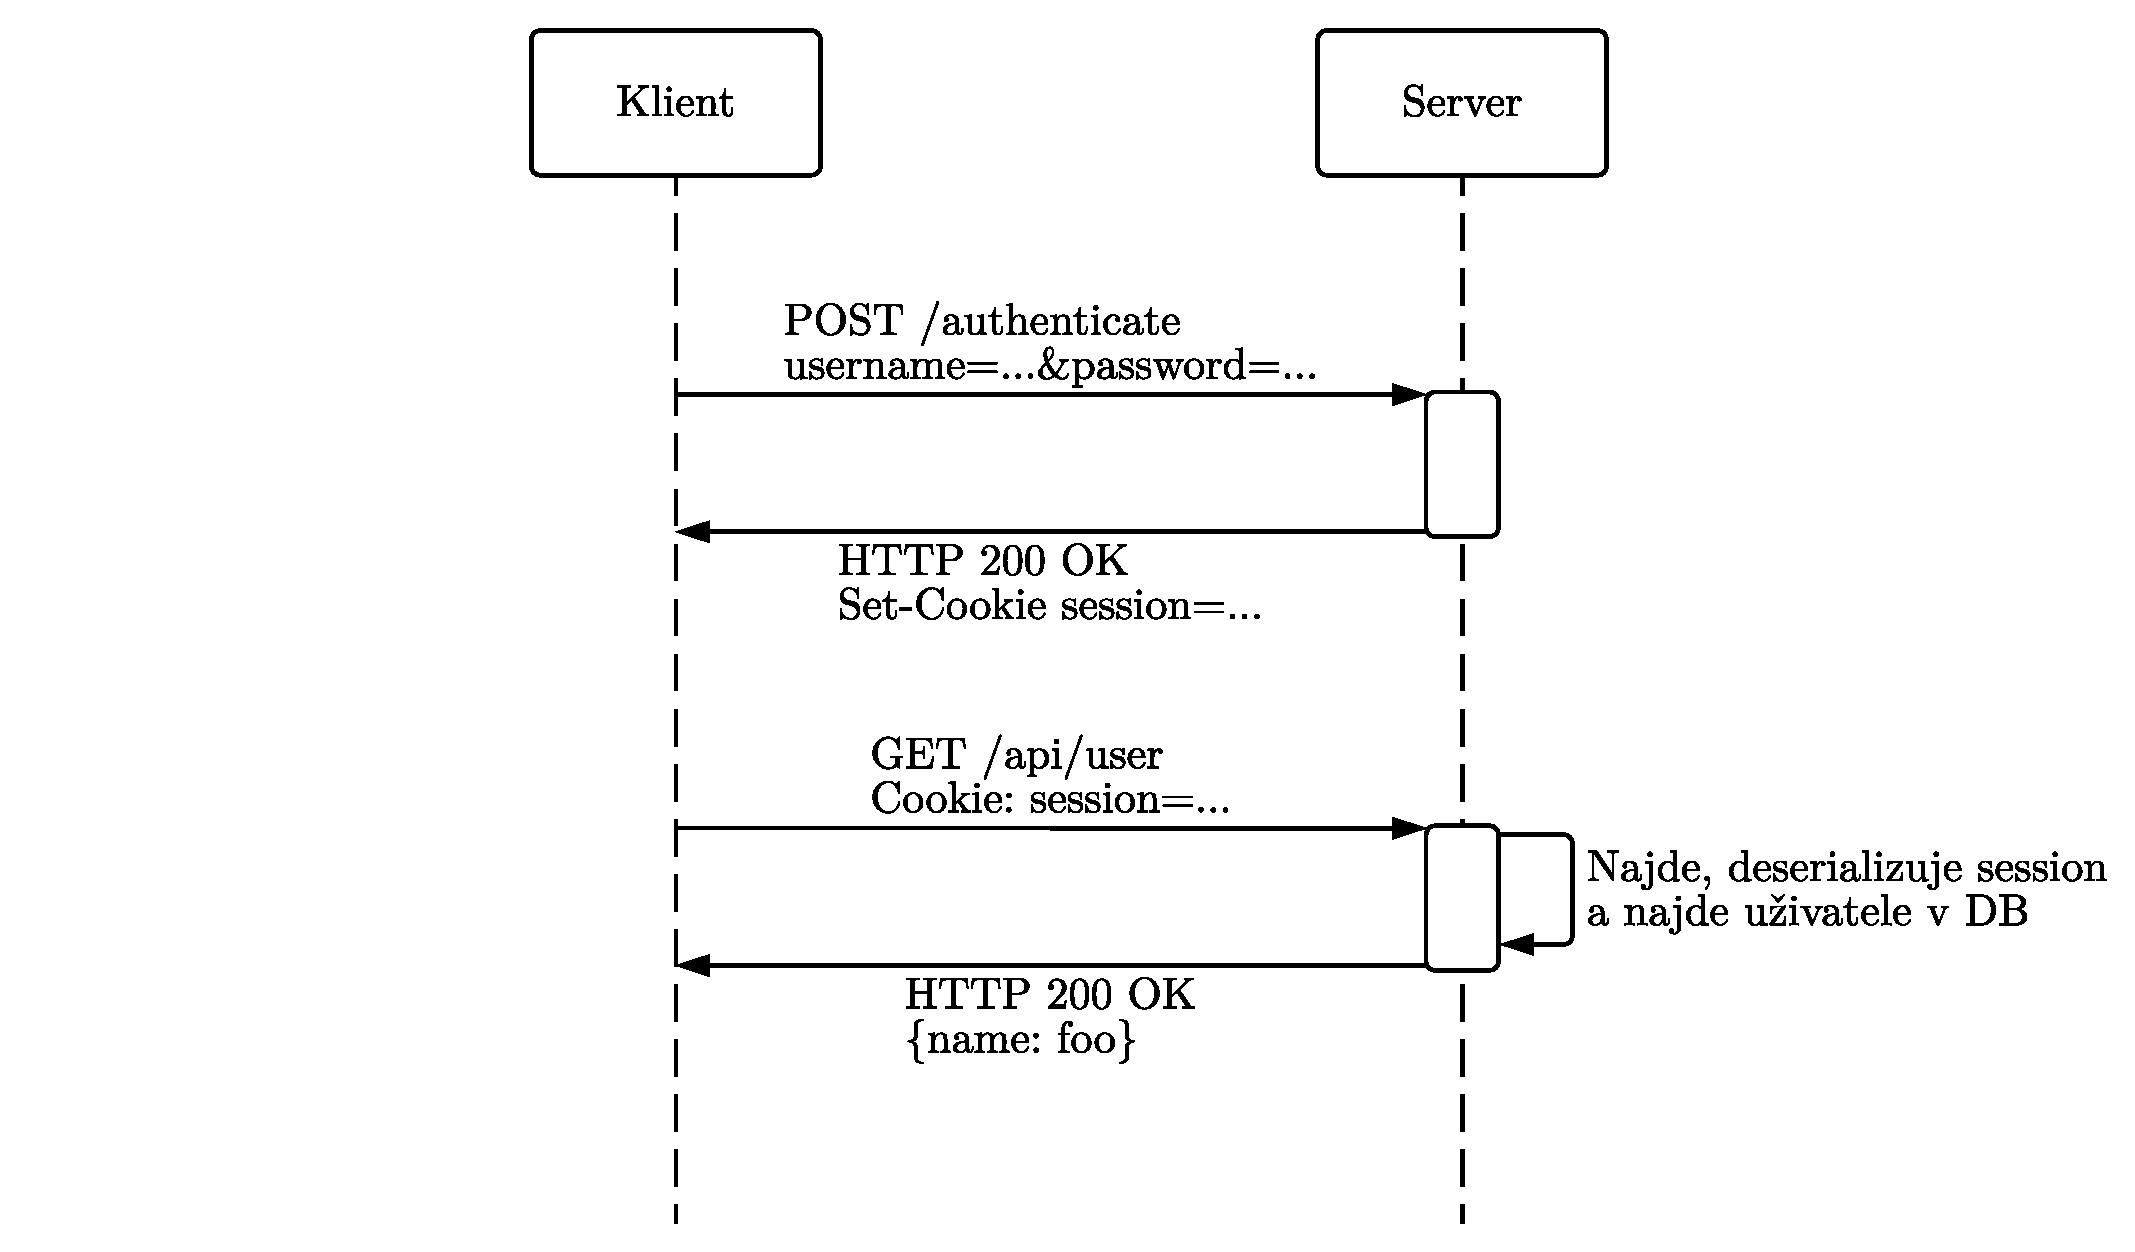
\includegraphics[width=\textwidth]{partials/navrh/statefullAuthentication.pdf}
    \caption{Sekvenční diagram stavové autentizace}\label{fig:statefullAuthentication}
\end{figure}

\subsection{Bezstavová autentizace}\label{subsec:bezstavováAutentizace}
Bezstavová autentizace (viz diagram na obrázku ~\ref{fig:statelessAuthentication}) je v poslední době velmi oblíbený způsob autentizace především pro \gls{REST} \gls{API}.
Autentizační server oproti nejčastěji přihlašovacím údajům vydává takzvaný token (speciální kód, který identifikuje uživatele).

Autentizační token samotný může nést více informací o uživateli, jako je například jeho jméno, ale také jeho oprávnění pro přístup ke zdrojům aplikace.
Díky tomu, že token nese informace o oprávnění nemusí, aplikační server při každém dotazu komunikovat s DB a zjišťovat uživatelovo oprávnění.
Bezstavová autentizace napomáhá škálování a rychlosti webových aplikací, ale je složitější na implementaci, jak na straně klient, tak na straně serveru.

\begin{figure}[ht!]
    \centering
    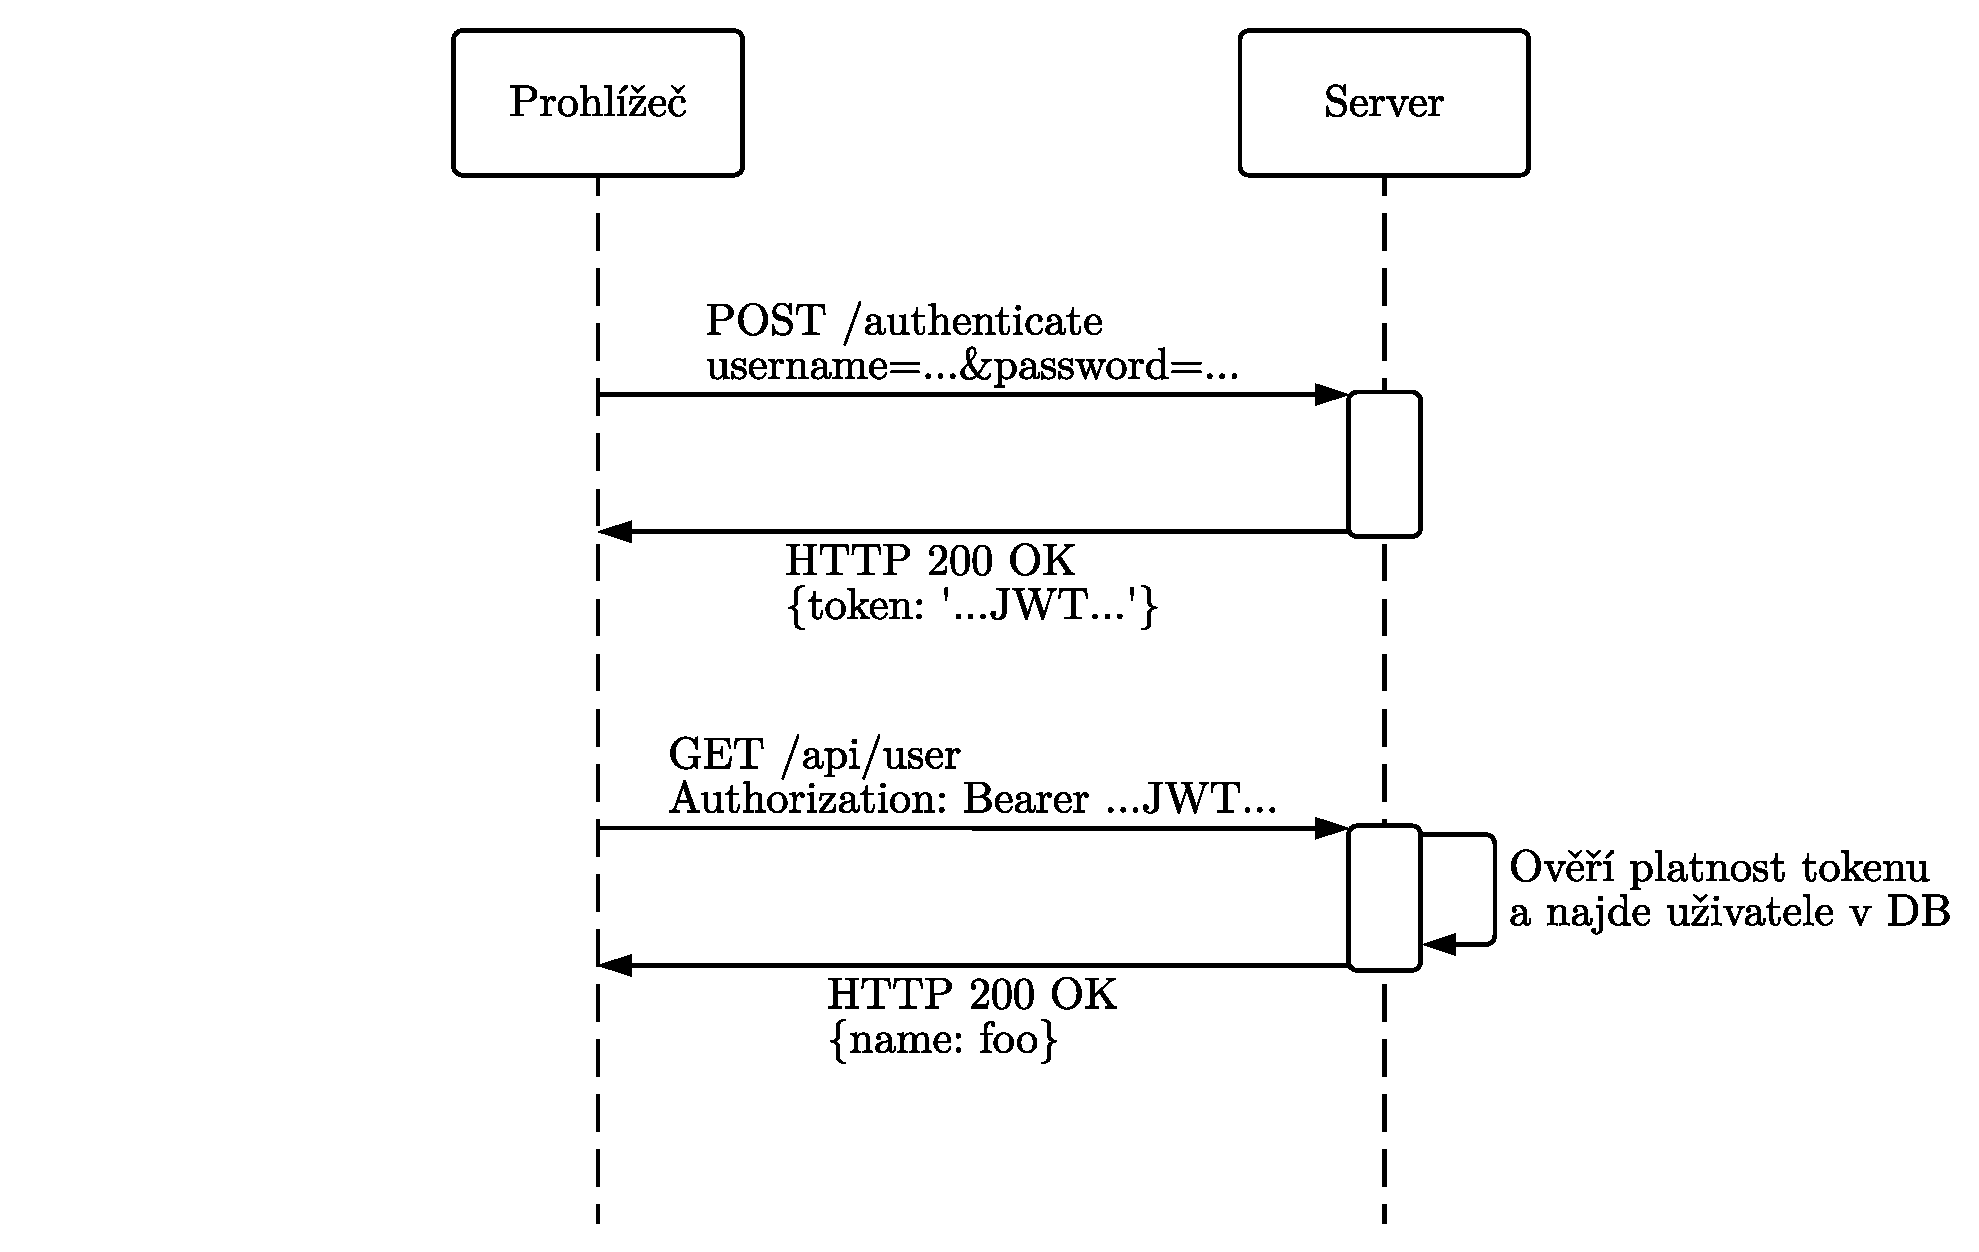
\includegraphics[width=\textwidth]{partials/navrh/statelessAuthentication.pdf}
    \caption{Sekvenční diagram bezstavové autentizace}\label{fig:statelessAuthentication}
\end{figure}

\subsection{Výběr způsobu autentizace}\label{subsec:výběrZpůsobuAutentizace}
Pro implementaci autentizace jsem se rozhodl použít jednoduchou stavovou autentizaci za pomoci klientského uložiště cookies a serverového uložiště session, které je perzistentně uloženo v DB.
Tento způsob jsem zvolil s ohledem na jednoduchost navrhovaného prototypu.

Díky stavové autentizaci nemusí klientská strana autentizaci vůbec řešit, protože prohlížeč odesílá platné cookies při každém požadavku automaticky.
To platí jak pro komunikaci pomocí \gls{REST} (viz následující sekce~\ref{sec:restKomunikace}), tak i pro komunikaci ve skutečném čase (viz následující sekce~\ref{sec:komunikaceVeSkutečnémČase}), kde se cookies odesílají při navázání spojení.
Nevýhodou tohoto řešení je, že obě části aplikace (klientská i serverová) musí být umístěny na stejné doméně.
V případě navrhovaného prototypu toto ale není problém, jelikož klientská i serverová část jsou sloučeny do jedné aplikace (viz sekce~\ref{sec:zveřejněníKlientskéČásti} o zveřejnění klientské části) a tudíž sdílí jednu společnou doménu.
